\documentclass{article}
\usepackage{iclr2027_conference,times}
\input{math_commands.tex}
\usepackage{hyperref}
\usepackage{url}
\usepackage{amsmath,amssymb,amsthm}
\usepackage{booktabs}
\usepackage{graphicx}
\usepackage{multirow}
\usepackage{xcolor}
\graphicspath{{figures/}}
% generated by exp/make_figures.py -- do not edit
\newcommand{\hwBaselineCZ}{2,027}
\newcommand{\hwBaselineFid}{0.20}
\newcommand{\hwBaselineSel}{0.19}
\newcommand{\hwFoldedCZ}{1,156}
\newcommand{\hwFoldedFid}{0.23}
\newcommand{\hwFoldedSel}{0.44}
\newcommand{\hwAqftCZ}{1,320}
\newcommand{\hwAqftFid}{0.23}
\newcommand{\hwAqftSel}{0.30}
\newcommand{\hwSemiclassicalCZ}{1,181}
\newcommand{\hwSemiclassicalFid}{0.24}
\newcommand{\hwSemiclassicalSel}{0.56}
\newcommand{\hwWindowedCZ}{699}
\newcommand{\hwWindowedFid}{0.40}
\newcommand{\hwWindowedSel}{0.71}
\newcommand{\speedClGPU}{169.63 ms}
\newcommand{\speedClGPUBatched}{0.672 ms}
\newcommand{\speedClGPUErr}{0.47}
\newcommand{\speedClCPU}{55.38 ms}
\newcommand{\speedClCPUErr}{0.47}
\newcommand{\speedQSim}{9.43 ms}
\newcommand{\speedQSimBatched}{0.088 ms}
\newcommand{\speedQSimErr}{0.58}
\newcommand{\speedQAer}{54 s}
\newcommand{\speedQAerErr}{0.58}
\newcommand{\speedHeron}{758 s}
\newcommand{\speedHeronZero}{188 s}
\newcommand{\speedHeronOrig}{17.0 h}
\newcommand{\speedCircuitsPerWindow}{1,140}
\newcommand{\speedAdaptiveShots}{2.9}
\newcommand{\speedAllThree}{8.0 s}
\newcommand{\speedPack}{14}
\newcommand{\fairClAdamErrSix}{0.588}
\newcommand{\fairClAdamRelSix}{+0.0}
\newcommand{\fairClAdamBetterSix}{0}
\newcommand{\fairClAdamPSix}{1.00}
\newcommand{\fairClAdamMsSix}{500.9}
\newcommand{\fairClAdamErrTwelve}{0.486}
\newcommand{\fairClAdamRelTwelve}{+0.0}
\newcommand{\fairClAdamBetterTwelve}{0}
\newcommand{\fairClAdamPTwelve}{1.00}
\newcommand{\fairClAdamMsTwelve}{43.5}
\newcommand{\fairClAdamFourErrSix}{0.631}
\newcommand{\fairClAdamFourRelSix}{+7.4}
\newcommand{\fairClAdamFourBetterSix}{8}
\newcommand{\fairClAdamFourPSix}{9\times10^{-52}}
\newcommand{\fairClAdamFourMsSix}{1.3}
\newcommand{\fairClAdamFourErrTwelve}{0.532}
\newcommand{\fairClAdamFourRelTwelve}{+9.5}
\newcommand{\fairClAdamFourBetterTwelve}{18}
\newcommand{\fairClAdamFourPTwelve}{4\times10^{-46}}
\newcommand{\fairClAdamFourMsTwelve}{3.1}
\newcommand{\fairClCoordErrSix}{0.607}
\newcommand{\fairClCoordRelSix}{+3.4}
\newcommand{\fairClCoordBetterSix}{36}
\newcommand{\fairClCoordPSix}{8\times10^{-37}}
\newcommand{\fairClCoordMsSix}{3.3}
\newcommand{\fairClCoordErrTwelve}{0.494}
\newcommand{\fairClCoordRelTwelve}{+1.8}
\newcommand{\fairClCoordBetterTwelve}{73}
\newcommand{\fairClCoordPTwelve}{4\times10^{-19}}
\newcommand{\fairClCoordMsTwelve}{6.0}
\newcommand{\fairClFineAdamErrSix}{0.588}
\newcommand{\fairClFineAdamRelSix}{+0.1}
\newcommand{\fairClFineAdamBetterSix}{163}
\newcommand{\fairClFineAdamPSix}{0.27}
\newcommand{\fairClFineAdamMsSix}{11.9}
\newcommand{\fairClFineAdamErrTwelve}{0.485}
\newcommand{\fairClFineAdamRelTwelve}{-0.2}
\newcommand{\fairClFineAdamBetterTwelve}{173}
\newcommand{\fairClFineAdamPTwelve}{0.15}
\newcommand{\fairClFineAdamMsTwelve}{30.5}
\newcommand{\fairClFineCoordErrSix}{0.604}
\newcommand{\fairClFineCoordRelSix}{+2.7}
\newcommand{\fairClFineCoordBetterSix}{62}
\newcommand{\fairClFineCoordPSix}{2\times10^{-30}}
\newcommand{\fairClFineCoordMsSix}{3.5}
\newcommand{\fairClFineCoordErrTwelve}{0.490}
\newcommand{\fairClFineCoordRelTwelve}{+0.9}
\newcommand{\fairClFineCoordBetterTwelve}{95}
\newcommand{\fairClFineCoordPTwelve}{2\times10^{-10}}
\newcommand{\fairClFineCoordMsTwelve}{6.4}
\newcommand{\fairQShiftErrSix}{0.638}
\newcommand{\fairQShiftRelSix}{+8.6}
\newcommand{\fairQShiftBetterSix}{22}
\newcommand{\fairQShiftPSix}{9\times10^{-48}}
\newcommand{\fairQShiftMsSix}{1.8}
\newcommand{\fairQShiftErrTwelve}{0.520}
\newcommand{\fairQShiftRelTwelve}{+7.1}
\newcommand{\fairQShiftBetterTwelve}{49}
\newcommand{\fairQShiftPTwelve}{6\times10^{-35}}
\newcommand{\fairQShiftMsTwelve}{3.9}
\newcommand{\fairQHwErrSix}{0.631}
\newcommand{\fairQHwRelSix}{+7.5}
\newcommand{\fairQHwBetterSix}{31}
\newcommand{\fairQHwPSix}{6\times10^{-45}}
\newcommand{\fairQHwMsSix}{2.1}
\newcommand{\fairQHwErrTwelve}{0.513}
\newcommand{\fairQHwRelTwelve}{+5.6}
\newcommand{\fairQHwBetterTwelve}{55}
\newcommand{\fairQHwPTwelve}{2\times10^{-29}}
\newcommand{\fairQHwMsTwelve}{4.8}
\newcommand{\fairQParityErrSix}{0.591}
\newcommand{\fairQParityRelSix}{+0.6}
\newcommand{\fairQParityBetterSix}{73}
\newcommand{\fairQParityPSix}{2\times10^{-10}}
\newcommand{\fairQParityMsSix}{4.6}
\newcommand{\fairQParityErrTwelve}{0.455}
\newcommand{\fairQParityRelTwelve}{-6.3}
\newcommand{\fairQParityBetterTwelve}{104}
\newcommand{\fairQParityPTwelve}{0.05}
\newcommand{\fairQParityMsTwelve}{8.6}
\newcommand{\fairN}{320}
\newcommand{\fairCoordVsHwBetterSix}{269}
\newcommand{\fairCoordVsHwPSix}{4\times10^{-35}}
\newcommand{\fairCoordVsHwRelSix}{-3.8}
\newcommand{\fairParityMedianDiffSix}{+0.030}
\newcommand{\fairRefFailSix}{21}
\newcommand{\fairCoordVsHwBetterTwelve}{264}
\newcommand{\fairCoordVsHwPTwelve}{2\times10^{-32}}
\newcommand{\fairCoordVsHwRelTwelve}{-3.6}
\newcommand{\fairParityMedianDiffTwelve}{+0.019}
\newcommand{\fairRefFailTwelve}{14}
\newcommand{\fairBfRefErrSix}{0.588}
\newcommand{\fairBfRefMedSix}{0.575}
\newcommand{\fairBfRefRelSix}{+0.0}
\newcommand{\fairBfRefBetterSix}{0}
\newcommand{\fairBfRefPSix}{1.00}
\newcommand{\fairBfRefErrTwelve}{0.486}
\newcommand{\fairBfRefMedTwelve}{0.437}
\newcommand{\fairBfRefRelTwelve}{+0.0}
\newcommand{\fairBfRefBetterTwelve}{0}
\newcommand{\fairBfRefPTwelve}{1.00}
\newcommand{\fairBfOneErrSix}{0.580}
\newcommand{\fairBfOneMedSix}{0.568}
\newcommand{\fairBfOneRelSix}{-1.2}
\newcommand{\fairBfOneBetterSix}{286}
\newcommand{\fairBfOnePSix}{3\times10^{-28}}
\newcommand{\fairBfOneErrTwelve}{0.479}
\newcommand{\fairBfOneMedTwelve}{0.430}
\newcommand{\fairBfOneRelTwelve}{-1.3}
\newcommand{\fairBfOneBetterTwelve}{244}
\newcommand{\fairBfOnePTwelve}{2\times10^{-16}}
\newcommand{\fairBfLowErrSix}{0.512}
\newcommand{\fairBfLowMedSix}{0.511}
\newcommand{\fairBfLowRelSix}{-12.9}
\newcommand{\fairBfLowBetterSix}{98}
\newcommand{\fairBfLowPSix}{4\times10^{-18}}
\newcommand{\fairBfLowErrTwelve}{0.398}
\newcommand{\fairBfLowMedTwelve}{0.387}
\newcommand{\fairBfLowRelTwelve}{-18.1}
\newcommand{\fairBfLowBetterTwelve}{125}
\newcommand{\fairBfLowPTwelve}{1\times10^{-22}}
\newcommand{\fairBfLowOneErrSix}{0.505}
\newcommand{\fairBfLowOneMedSix}{0.503}
\newcommand{\fairBfLowOneRelSix}{-14.1}
\newcommand{\fairBfLowOneBetterSix}{295}
\newcommand{\fairBfLowOnePSix}{7\times10^{-39}}
\newcommand{\fairBfLowOneErrTwelve}{0.391}
\newcommand{\fairBfLowOneMedTwelve}{0.379}
\newcommand{\fairBfLowOneRelTwelve}{-19.6}
\newcommand{\fairBfLowOneBetterTwelve}{278}
\newcommand{\fairBfLowOnePTwelve}{5\times10^{-36}}
\newcommand{\fairBfParityErrSix}{0.591}
\newcommand{\fairBfParityMedSix}{0.595}
\newcommand{\fairBfParityRelSix}{+0.6}
\newcommand{\fairBfParityBetterSix}{73}
\newcommand{\fairBfParityPSix}{2\times10^{-10}}
\newcommand{\fairBfParityErrTwelve}{0.455}
\newcommand{\fairBfParityMedTwelve}{0.447}
\newcommand{\fairBfParityRelTwelve}{-6.3}
\newcommand{\fairBfParityBetterTwelve}{104}
\newcommand{\fairBfParityPTwelve}{0.05}
\newcommand{\fairDriftFailSix}{79}
\newcommand{\fairDriftOKSix}{9}
\newcommand{\fairLowVsParityRelSix}{-13.3}
\newcommand{\fairLowVsParityBetterSix}{301}
\newcommand{\fairLowVsParityPSix}{4\times10^{-47}}
\newcommand{\fairLowBfVsParityRelSix}{-14.6}
\newcommand{\fairLowBfVsParityBetterSix}{301}
\newcommand{\fairLowBfVsParityPSix}{2\times10^{-47}}
\newcommand{\fairLowFailSix}{0}
\newcommand{\fairDriftFailTwelve}{84}
\newcommand{\fairDriftOKTwelve}{11}
\newcommand{\fairLowVsParityRelTwelve}{-12.6}
\newcommand{\fairLowVsParityBetterTwelve}{289}
\newcommand{\fairLowVsParityPTwelve}{2\times10^{-39}}
\newcommand{\fairLowBfVsParityRelTwelve}{-14.2}
\newcommand{\fairLowBfVsParityBetterTwelve}{285}
\newcommand{\fairLowBfVsParityPTwelve}{1\times10^{-38}}
\newcommand{\fairLowFailTwelve}{0}
\newcommand{\cohNumpyDiff}{1e-16}
\newcommand{\cohQiskitDiff}{8e-10}
\newcommand{\cohSuccess}{0.307}
\newcommand{\cohReflCZ}{254}
\newcommand{\cohK}{4}
\newcommand{\cohN}{64}
\newcommand{\cohSetCEight}{0.43}
\newcommand{\cohSetCSixteen}{0.29}
\newcommand{\cohSetCTwentyFour}{0.21}
\newcommand{\cohSetCThirtyTwo}{0.16}
\newcommand{\qpuBackend}{prediction only}
\newcommand{\qpuN}{26}
\newcommand{\qpuShots}{4,000}
\newcommand{\qpuJobs}{--}
\newcommand{\qpuShortN}{24}
\newcommand{\qpuShortPeakOK}{19}
\newcommand{\qpuShortSel}{0.98}
\newcommand{\qpuShortSelMin}{0.91}
\newcommand{\qpuShortFid}{0.86}
\newcommand{\qpuShortFidSim}{0.86}
\newcommand{\qpuShortTVD}{0.23}
\newcommand{\qpuDynFid}{0.88}
\newcommand{\qpuDynSel}{0.99}
\newcommand{\qpuDynPeakOK}{10}
\newcommand{\qpuDynN}{12}
\newcommand{\qpuDynCZ}{216}
\newcommand{\qpuUniFid}{0.85}
\newcommand{\qpuUniSel}{0.98}
\newcommand{\qpuUniPeakOK}{9}
\newcommand{\qpuUniN}{12}
\newcommand{\qpuUniCZ}{272}
\newcommand{\qpuLongFid}{0.39}
\newcommand{\qpuLongSel}{0.32}
\newcommand{\qpuLongPeakOK}{0}
\newcommand{\qpuLongCZ}{1166}
\newcommand{\qpuSeconds}{0}

\InputIfFileExists{numbers_denoise.tex}{}{}
% device macros are defined by numbers.tex once the QPU run has been folded in
\providecommand{\qpuBackend}{ibm\_marrakesh}
\providecommand{\qpuN}{--}\providecommand{\qpuShots}{--}\providecommand{\qpuJobs}{--}
\providecommand{\qpuShortN}{--}\providecommand{\qpuShortPeakOK}{--}\providecommand{\qpuShortSel}{--}
\providecommand{\qpuShortSelMin}{--}\providecommand{\qpuShortFid}{--}\providecommand{\qpuShortFidSim}{--}
\providecommand{\qpuShortTVD}{--}\providecommand{\qpuDynFid}{--}\providecommand{\qpuDynSel}{--}
\providecommand{\qpuDynPeakOK}{--}\providecommand{\qpuDynN}{--}\providecommand{\qpuDynCZ}{--}
\providecommand{\qpuUniFid}{--}\providecommand{\qpuUniSel}{--}\providecommand{\qpuUniPeakOK}{--}
\providecommand{\qpuUniN}{--}\providecommand{\qpuUniCZ}{--}\providecommand{\qpuLongFid}{--}
\providecommand{\qpuLongSel}{--}\providecommand{\qpuLongPeakOK}{--}\providecommand{\qpuLongCZ}{--}
\providecommand{\qpuSeconds}{--}
\providecommand{\fairBfRefErrSix}{--}\providecommand{\fairBfOneErrSix}{--}\providecommand{\fairBfLowErrSix}{--}
\providecommand{\fairBfLowOneErrSix}{--}\providecommand{\fairBfParityErrSix}{--}
\providecommand{\fairBfRefErrTwelve}{--}\providecommand{\fairBfOneErrTwelve}{--}\providecommand{\fairBfLowErrTwelve}{--}
\providecommand{\fairBfLowOneErrTwelve}{--}\providecommand{\fairBfParityErrTwelve}{--}
\providecommand{\fairBfOneRelSix}{--}\providecommand{\fairBfOneRelTwelve}{--}
\providecommand{\fairBfLowRelSix}{--}\providecommand{\fairBfLowRelTwelve}{--}
\providecommand{\fairBfLowOneRelSix}{--}\providecommand{\fairBfLowOneRelTwelve}{--}
\providecommand{\fairBfOneBetterSix}{--}\providecommand{\fairBfOneBetterTwelve}{--}
\providecommand{\fairBfLowBetterSix}{--}\providecommand{\fairBfLowBetterTwelve}{--}
\providecommand{\fairBfLowOneBetterSix}{--}\providecommand{\fairBfLowOneBetterTwelve}{--}
\providecommand{\fairBfOnePSix}{--}\providecommand{\fairBfOnePTwelve}{--}
\providecommand{\fairBfLowPSix}{--}\providecommand{\fairBfLowPTwelve}{--}
\providecommand{\fairBfLowOnePSix}{--}\providecommand{\fairBfLowOnePTwelve}{--}
\providecommand{\fairDriftFailSix}{--}\providecommand{\fairDriftOKSix}{--}
\providecommand{\fairDriftFailTwelve}{--}\providecommand{\fairDriftOKTwelve}{--}
\providecommand{\fairLowVsParityRelSix}{--}\providecommand{\fairLowVsParityBetterSix}{--}\providecommand{\fairLowVsParityPSix}{--}
\providecommand{\fairLowVsParityRelTwelve}{--}\providecommand{\fairLowVsParityBetterTwelve}{--}\providecommand{\fairLowVsParityPTwelve}{--}
\providecommand{\fairLowBfVsParityRelSix}{--}\providecommand{\fairLowBfVsParityBetterSix}{--}\providecommand{\fairLowBfVsParityPSix}{--}
\providecommand{\fairLowBfVsParityRelTwelve}{--}\providecommand{\fairLowBfVsParityBetterTwelve}{--}\providecommand{\fairLowBfVsParityPTwelve}{--}
\providecommand{\fairLowFailSix}{--}\providecommand{\fairLowFailTwelve}{--}
\providecommand{\fairBfParityRelSix}{--}\providecommand{\fairBfParityRelTwelve}{--}
\providecommand{\fairBfParityBetterSix}{--}\providecommand{\fairBfParityBetterTwelve}{--}
\providecommand{\fairBfParityPSix}{--}\providecommand{\fairBfParityPTwelve}{--}

\newtheorem{proposition}{Proposition}
\newcommand{\qact}{QACT}
\newcommand{\act}{ACT}
\newcommand{\ket}[1]{\lvert #1\rangle}
\newcommand{\bra}[1]{\langle #1\rvert}
\newcommand{\braket}[2]{\langle #1\,|\,#2\rangle}
\newcommand{\norm}[1]{\lVert #1\rVert}

\title{A Quantum Chirplet Transform, Audited:\\ Exact Circuits, Fair Controls, and a Real-Device Test}

% Submission is double blind; the author block is filled in for the camera-ready only.
\author{Anonymous authors\\ Paper under double-blind review}

%\iclrfinalcopy % camera-ready only
\begin{document}
\maketitle

\begin{abstract}
Quantum machine learning for time series usually places the quantum component downstream of a classical representation. We put it inside the representation. The adaptive chirplet transform (\act) writes a signal as a few Gaussian-windowed linear chirps chosen by matching pursuit; because a chirp's quadratic phase is exactly 2-local in the binary encoding of time, a chirplet atom is an $O(n^2)$-gate circuit on $n=\log_2 N$ qubits, one quantum Fourier transform returns the atom's whole frequency axis at once, measurement samples atoms with probability proportional to the correlation matching pursuit maximises, and the parameter-shift rule refines every phase parameter exactly. We call the result the quantum \act\ (\qact) and audit it as a classical method would be audited. Every function of a strong classical engine is reproduced in quantum-native form, and the distribution a device actually reports, conditioned on post-selection, turns out to be the classical normalised selection criterion. On real EEG, in pre-registered comparisons with paired tests, every apparent \qact\ advantage had a classical explanation: the transform's free 0.5\,Hz frequency axis, and a classical seed band that excludes the mains interference the transform can represent. We run the controls that isolate each, including the one that looked like a refiner effect and was not, and find the classical engine at least as good at equal function set; downstream, quantum kernels, variational classifiers, quantum recurrent models and quantum reservoirs land at parity or below on seizure detection across 37 patients and forecasting for 23 people, while the chirplet features themselves add 9--13 accuracy points. We give the exact dequantisation of the sampler (a periodogram, $O(N\log N)$) and identify what survives it: the dictionary is gate-native and needs no QRAM, and the matching-pursuit residual can be kept coherent by a one-ancilla reflection whose success probability is exactly the residual energy fraction, which we verify on circuits. On an IBM Heron processor, folding the envelope into state preparation, a semiclassical QFT and window-local registers reduce a short atom's circuit from 2,027 to about 140 two-qubit gates, and on the device the six-qubit circuits select the atom the exact distribution selects in \qpuSixPeakOK\ of \qpuSixN\ cases and never fall below \qpuSixSelMin\ of the best atom's energy, seven-qubit circuits are marginal, and long atoms do not survive. A fully controlled parity result is, we argue, the baseline any quantum advantage for recorded signals has to clear.
\end{abstract}

\section{Introduction}
Sparse time--frequency representations are the workhorse of biomedical signal analysis. The adaptive chirplet transform (\act) of \citet{mann1991chirplet,mann1992adaptive,mann1995chirplet} represents a signal as a sum of Gaussian-windowed linear-frequency-modulated atoms selected greedily by matching pursuit \citep{mallat1993matching,bultan1999four}; the chirp rate is the parameter a stationary spectrum cannot report, and it is what makes the representation informative for drifting EEG transients. Proposals to accelerate such decompositions on quantum hardware exist \citep{bellante2022qmp,bellante2025qomp}, but they assume quantum random-access memory for both the signal and the dictionary, and they have not been run on data.

This paper studies a quantum \act\ built from one observation: the chirplet atom is itself a shallow circuit. Writing the time index in binary, $t=\sum_k b_k 2^k$ with $b_k^2=b_k$, the quadratic phase $\exp(i2\pi c t^2/N)$ factorises into $n$ single-qubit and $n(n-1)/2$ two-qubit phase gates exactly, the linear phase into $n$ single-qubit gates, and the Gaussian envelope is a diagonal filter. After the conjugate chirp and an inverse quantum Fourier transform, the amplitude on frequency bin $k$ is the correlation $\braket{\psi_{\theta}}{x}$ of the signal with the atom $\theta=(t_c,f_c,\Delta t,c)$, so the frequency axis of the dictionary is read out by one transform and \emph{measurement samples atoms with the probability matching pursuit maximises}. The parameter-shift rule \citep{mitarai2018circuit,schuld2019evaluating} is exact for every phase parameter, because the captured energy is a degree-one trigonometric polynomial in every gate angle.

We do not claim an advantage. We ask the question a reviewer of any new representation would ask: \emph{when the quantum version is implemented with every function of its classical peer, does it learn or reconstruct anything the classical one does not, and if not, why not?} Answering it required more care than expected. \qact\ first appeared to win on denoising against ICA-cleaned ground truth (better on 17 of 18 held-out subjects, $p<10^{-4}$); no bug produced the win, but it was the transform's finer frequency grid, which the classical engine can copy. A hardware-motivated coordinate-search refiner then appeared to beat the frequency-matched classical engine; giving the classical engine the same refiner does \emph{not} close that gap, and letting its seed grid reach the 50\,Hz mains the artifact injection contains does. On public data the classical engine failed on windows dominated by 60\,Hz mains that its 40\,Hz seed grid excludes, which made \qact\ look better in the mean but not the median. Each effect is a legitimate engineering finding; none is a quantum one.

\paragraph{Contributions.}
(1) A quantum \act\ with exact circuits for the atom, the selection step and the refinement gradient, brought to full functional parity with a strong classical engine (\S\ref{sec:qact}), including the observation that the post-selection-conditioned distribution a device reports \emph{is} the classical normalised criterion, which fixed a 70\% deficit.
(2) A pre-registered audit on real EEG (\S\ref{sec:exp}): denoising with ground truth on 26 subjects, seizure detection on 37 patients of two databases, per-person forecasting on 983 hours, with the controls that dissolved each apparent advantage, three of them run for this paper.
(3) The exact dequantisation of the sampler and a precise account of what quantum structure survives it (\S\ref{sec:theory}): a gate-native dictionary that needs no QRAM, and a coherent residual update with success probability equal to the residual energy fraction, verified on circuits to $10^{-9}$.
(4) The first execution of the transform's selection step on a quantum processor (\S\ref{sec:hw}): circuit constructions that cut a short atom from 2,027 to about 140 CZ gates, and device histograms that select the exact atom at six qubits, degrade at seven, and fail for long atoms, with job identifiers and the classical certificate for each.
Code, per-window records and the pre-registered comparisons are released.

\section{Background}
\paragraph{The transform.} Let $x\in\mathbb{R}^N$, $N=2^n$. A chirplet atom in the sample domain is
\begin{equation}
\psi_\theta(t)=\frac{1}{\norm{\psi_\theta}}\,e^{-(t-t_c)^2/2\Delta t^2}\,\exp\!\Big(\tfrac{i2\pi}{N}\big[c\,(t-t_c)^2+f_c\,(t-t_c)\big]\Big),\qquad \theta=(t_c,f_c,\Delta t,c),
\label{eq:atom}
\end{equation}
with $f_c$ in cycles per window and $c$ in cycles per window per sample. Matching pursuit picks the atom maximising $|\braket{\psi_\theta}{r}|^2$ against the residual $r$, refines $\theta$ off-grid, subtracts, and repeats; orthogonal matching pursuit (OMP) re-fits all coefficients jointly \citep{pati1993omp}. The classical engine used throughout is a batched GPU implementation of the \act\ of \citet{actcode}: a 20,400-atom seed grid (17 centres $\times$ 40 frequencies at 1\,Hz $\times$ 6 widths $\times$ 5 chirp rates), the least-squares energy of the cosine/sine quadrature pair as selection criterion, sixty steps of Adam on the same objective as refinement, OMP, and a per-window stopping rule. We refer to it as the classical engine; a two-width asymmetric envelope \citep{actcode} is available as a variant.

\paragraph{Quantum learning on EEG.} Quantum kernels \citep{havlicek2019supervised,huang2021power}, re-uploading classifiers \citep{perez2020reuploading}, quantum recurrent models \citep{chen2020qlstm} and quantum reservoirs \citep{fujii2017harnessing,martinez2021dynamical} have all been applied to biosignals, usually on features a classical transform produced. \citet{bowles2024better} showed that most reported quantum-versus-classical wins in learning do not survive matched baselines; \citet{wolff2026qrc} found a quantum reservoir that wins on benchmarks and loses on EEG. Our audit follows that discipline and moves it one step upstream, into the representation.

\section{The quantum adaptive chirplet transform}
\label{sec:qact}
\subsection{The atom is a circuit}
Expanding $c(t-t_c)^2+f_c(t-t_c)=c\,t^2+(f_c-2ct_c)\,t+\text{const}$ shows that a shifted chirp is the same quadratic phase plus a linear phase at the \emph{effective frequency} $f=f_c-2ct_c$; the centre time enters only through the envelope. With $t=\sum_k b_k2^k$,
\begin{equation}
t^2=\sum_k b_k 2^{2k}+2\sum_{j<k}b_jb_k2^{j+k}
\;\Rightarrow\;
e^{i2\pi ct^2/N}=\prod_k P_k\!\big(\tfrac{2\pi c\,2^{2k}}{N}\big)\prod_{j<k}CP_{jk}\!\big(\tfrac{2\pi c\,2^{j+k+1}}{N}\big),
\label{eq:twolocal}
\end{equation}
a product of $n$ phase gates and $n(n-1)/2$ controlled-phase gates, exactly \citep[verified against the analytic diagonal and against a statevector simulation to $9\times10^{-13}$ and $4\times10^{-14}$;][]{qiskit2024}. A cubic phase $e^{i2\pi c_3t^3/N}$, an atom whose chirp rate itself evolves, is 3-local by the same argument (129 gates at $n=9$). The Gaussian envelope is a real diagonal filter, realised either by a multiplexed rotation onto an ancilla with post-selection or, as we do on hardware, by folding it into state preparation (\S\ref{sec:hw}).

\subsection{Selection by one transform and one measurement}
Prepare $\ket{s}$ with $s=e\odot r/\norm{e\odot r}$ for envelope $e=e_{t_c,\Delta t}$, apply the conjugate chirp for rate $c$ and an inverse QFT, and measure the register. The outcome $k$ has probability
\begin{equation}
P_{e,c}(k)=\frac{1}{N}\Big|\sum_t s(t)\,e^{-i2\pi ct^2/N}e^{-i2\pi kt/N}\Big|^2,
\label{eq:sampler}
\end{equation}
which, rescaled by the classical factor $N\norm{e\odot r}^2/\norm{e}^2$, equals $|\braket{\psi_{e,c,k}}{r}|^2/\norm{\psi}^2$, the energy of atom $(t_c,\Delta t,c,k)$ captured from $r$, normalised by the atom's norm. Every frequency of the dictionary for one $(t_c,\Delta t,c)$ triple is therefore covered by a single circuit; the remaining triples are enumerated (one circuit each) or, in principle, superposed in index registers and searched by quantum maximum finding \citep{durr1996minimum} (\S\ref{sec:theory}). Sampling the outcome makes selection stochastic; the argmax over the identical dictionary is the control that isolates measurement from formulation, and \texttt{shots} interpolates between the two.

The normalisation in the previous sentence was the source of the transform's first failure. The raw histogram is the \emph{joint} probability that the envelope filter succeeds and frequency $k$ is read, so it over-ranks wide, high-norm envelopes. A device keeps only post-selected shots, so what it reports is the \emph{conditional} distribution; dividing by the filter's success probability $\norm{\psi}^2$ makes the hardware observable, the refiner's objective and the classical least-squares criterion the same quantity. This one change moved \qact\ from a reconstruction error of 0.307 to 0.169 on planted chirplets and, on real EEG denoising, from 70\% worse than the classical engine to statistically indistinguishable from it (\S\ref{sec:denoise}).

\subsection{Exact refinement by the parameter-shift rule}
The captured energy $E(\theta)=|\braket{\psi_\theta}{r}|^2/\norm{\psi_\theta}^2$ depends on every phase-gate angle $a$ through a factor $e^{ia}$ multiplying part of the overlap, so $E=A+B\cos a+C\sin a$ and $\partial E/\partial a=[E(a+\pi/2)-E(a-\pi/2)]/2$ exactly \citep{mitarai2018circuit,schuld2019evaluating}. The chain rule maps the $n+n(n-1)/2$ angles onto $f$ and $c$ with the weights of eq.~\eqref{eq:twolocal}; the envelope parameters are not gate angles and use central differences, as a device would. Closed-form and genuinely shifted evaluations agree to $2.8\times10^{-9}$; each step costs 112 circuit evaluations, and four steps cut reconstruction error on planted signals by about 25\%. A cheaper rule, used on hardware, is a three-point coordinate search (two evaluations per coordinate, keep the best of three) at 8 evaluations per step; it scores \emph{better} than the gradient on denoising, an effect we later have to explain (\S\ref{sec:denoise}).

\subsection{Functional parity}
\label{sec:parity}
A transform that only selects atoms is not the classical engine. Table~\ref{tab:parity} lists every function of the classical engine and its quantum-native counterpart; each is opt-in, and with all of them off the transform reproduces the pre-parity reference feature matrix bit for bit (2.5 million entries). The OMP refit costs no circuits: its normal matrix is the Gram matrix of atom overlaps $\braket{\psi_i}{\psi_j}$, which is a swap-test observable in principle but depends only on atom parameters, so both it and the right-hand side are classical. The exact frequency update follows from eq.~\eqref{eq:sampler}: $E(f)$ is the periodogram, so the optimal $f$ is read off one transform instead of gradient-stepped toward. Two functions have no classical counterpart in the engine we compare against (the exact frequency update and backfit), and the control study of \S\ref{sec:control} therefore adds backfit to the classical engine as well.

\begin{table}[t]
\caption{Functional parity between the classical engine and \qact. ``Cost'' is what the function costs on a device beyond the selection circuit.}
\label{tab:parity}
\centering\small
\resizebox{\textwidth}{!}{%
\begin{tabular}{@{}lll@{}}
\toprule
classical engine & \qact\ & cost on a device \\
\midrule
dictionary search, least-squares energy & one circuit per $(t_c,\Delta t,c)$; histogram conditioned on post-selection & shots \\
Adam refinement of $(t_c,f_c,\log\Delta t,c)$ & parameter shift for phases, central differences for envelope & 112 evaluations/step \\
& \quad or three-point coordinate search & 8 evaluations/step \\
OMP joint refit & Gram of atom overlaps; parameters known, so classical & none \\
two-width asymmetric envelope & fourth envelope grid axis, refinable & none \\
stopping rule (active mask) & same semantics & none \\
-- & exact frequency update (periodogram read-out) & one circuit \\
-- & backfit: cyclic re-refinement of each atom & refinement $\times$ atoms \\
-- & cubic phase (3-local) and skew envelope, refinable & 129 gates at $n=9$ \\
\bottomrule
\end{tabular}}
\end{table}

\section{What the quantum structure buys, exactly}
\label{sec:theory}
\begin{proposition}[Exact sampler and its dequantisation]
\label{prop:dequant}
For any envelope $e$, chirp rate $c$ and residual $r$, the outcome distribution of the selection circuit is eq.~\eqref{eq:sampler}, and $N\norm{e\odot r}^2\norm{e}^{-2}P_{e,c}(k)=|\braket{\psi_{e,c,k}}{r}|^2/\norm{\psi_{e,c,k}}^2$ for every $k$. All $N$ values are computed classically by one fast Fourier transform of $e\odot r\odot e^{-i2\pi ct^2/N}$ in $O(N\log N)$ operations.
\end{proposition}
The proof is the definition of the QFT (Appendix~\ref{app:proofs}). The consequence is that an \emph{enumerated} \qact\ with $S$ shots per triple costs $\Theta(M'\,S\,N)$ gate-time per iteration (state preparation of an arbitrary $N$-vector needs $\Theta(N)$ gates without QRAM \citep{mottonen2005transformation,shende2006synthesis}) against $\Theta(M'N\log N)$ classical operations, and that a classical program that computes eq.~\eqref{eq:sampler} by FFT and takes the argmax is exactly the transform with infinitely many shots. We ran that program: on the GPU it decomposes a window in \speedQSimBatched\ (batched), faster than the classical engine (\speedClGPUBatched) because it uses four cheap refinement steps instead of sixty, at a worse fit (\speedQSimErr\ versus \speedClGPUErr). It is a classical algorithm that computes what the circuit would.

Two pieces of quantum structure are not dequantised by Proposition~\ref{prop:dequant}. The first is that the dictionary is \emph{gate-native}: an atom is $O(n^2)$ gates plus a Gaussian preparation \citep{grover2002creating}, so a superposition over the $M'$ triples in index registers costs controlled versions of those gates, not a QRAM of $M'N$ amplitudes as quantum matching pursuit assumes \citep{bellante2022qmp,jaques2025qram}. Quantum maximum finding over the index registers then selects the best triple in $O(\sqrt{M'})$ evaluations \citep{durr1996minimum,brassard2002amplitude}. The second is the residual.

\begin{proposition}[Coherent residual]
\label{prop:coherent}
Let $P_k=I-\ket{\psi_k}\bra{\psi_k}$ and $R_k=I-2\ket{\psi_k}\bra{\psi_k}=U_k(I-2\ket{0}\bra{0})U_k^\dagger$, where $U_k\ket{0}=\ket{\psi_k}$ is the atom's preparation circuit. With one ancilla, $(H\otimes I)\,\mathrm{c}\text{-}R_k\,(H\otimes I)$ applied to $\ket{0}\ket{r}$ and post-selected on the ancilla reading $0$ yields $P_k\ket{r}$ with probability $\norm{P_kr}^2/\norm{r}^2$. Chaining $K$ such steps on the loaded signal $\ket{x}$ yields exactly the classical matching-pursuit residual $r_K$, with success probability $\norm{r_K}^2/\norm{x}^2$, the fraction of the signal's energy the $K$ atoms leave unexplained.
\end{proposition}
The proof is two lines (Appendix~\ref{app:proofs}); we verified it on a real EEG window with $N=\cohN$ and $K=\cohK$: the chained projectors match the classical residual to $\cohNumpyDiff$ in a numpy statevector and to $\cohQiskitDiff$ in a circuit built from state preparation, phase gates and a multi-controlled phase, with success probability $\cohSuccess$ equal to $\norm{r_K}^2/\norm{x}^2$ to six digits. One controlled reflection costs \cohReflCZ\ two-qubit gates at $n=6$ on an all-to-all CZ basis, dominated by the two envelope preparations. On the 320 public EEG windows of \S\ref{sec:control}, the success probability is $\cohSetCEight$, $\cohSetCSixteen$, $\cohSetCTwentyFour$ and $\cohSetCThirtyTwo$ at 8, 16, 24 and 32 atoms (Fig.~\ref{fig:coherent}, Appendix~\ref{app:proofs}): the algorithm slows down precisely as it succeeds, and amplitude amplification keeps the repetition count between two and three.

What the coherent residual removes is the classical computation of $r_k$ between iterations, not the $\Theta(N)$ load of $x$, which every Grover repetition must repeat. The honest complexity of the superposed variant without QRAM is therefore $O\big(\sqrt{M'}\,\varepsilon^{-1}(N+Kn^2)\big)$ gate-time per iteration for amplitude resolution $\varepsilon$, against $O(M'N\log N)$ classically: polynomial in the dictionary size only, and eaten at the dictionary sizes EEG needs ($M'\le 5{,}000$) by the clock-speed and shot costs measured in \S\ref{sec:hw}. With coherent access to the signal (QRAM, or a signal that reaches a qubit directly, \citealp{huang2022advantage,kannan2026exponential}), the same construction runs in $O(\sqrt{M'}\varepsilon^{-1}(Kn^2+\mathrm{polylog}\,N))$, which is the regime the quantum matching-pursuit literature analyses. The dequantisation literature \citep{aaronson2015fineprint,tang2019quantum,chia2020sampling,tang2022dequantizing} predicts exactly this split, and the experiments below are consistent with it.


\section{Experiments on real EEG}
\label{sec:exp}
\paragraph{Protocol.} Every comparison was pre-registered with its decision rule before it was run: subject-wise or patient-wise folds, paired Wilcoxon signed-rank tests across subjects or patients, and Bonferroni correction over the tests run on a dataset. The two frequency-matched denoising arms were added after the parity result was seen and were named as the deciding controls before they ran. Negative results are reported in place. Datasets: EEGMAT \citep{zyma2019eegmat}, 36 subjects, ICA-cleaned by its authors, 500\,Hz resampled to 256\,Hz; CHB-MIT \citep{shoeb2009application}, 23 cases of 22 paediatric patients, 198 seizures, 983\,h; the Siena scalp EEG database \citep{detti2020siena}, 14 patients, 45 seizures, used once as a confirmation set; and, for the controls added in this paper, the PhysioNet EEG motor movement/imagery baseline runs \citep{schalk2004bci2000,goldberger2000physionet}, 20 subjects, read with MNE \citep{gramfort2013mne}. All data are public \citep{goldberger2000physionet}.

\subsection{Denoising against ground truth}
\label{sec:denoise}
Reconstruction error cannot measure denoising, because leaving noise in the residual is what a denoiser should do. EEGMAT is ICA-cleaned, so it serves as a clean reference: known artifacts (blinks, horizontal eye movement, EMG, the subject's own ECG, electrode pops, mains, drift, with per-channel propagation) are injected, each engine decomposes the corrupted signal, atoms flagged as artifact by an amplitude-gated rule are dropped, and the rebuilt signal is scored against the clean one by a time-domain fidelity plus per-band power error in dB. Thresholds are tuned on eight subjects and frozen; 18 others are held out (26 of the 36 subjects are used). Table~\ref{tab:denoise} gives the arms.

\begin{table}[t]
\caption{EEGMAT denoising, 18 held-out subjects: score (lower is better; time fidelity plus per-band dB error), relative RMSE, delta-band error, and the paired comparison. Bonferroni $\alpha=0.0056$ (nine tests) for the first block, $0.0125$ (four) for the second and for the two arms run for this paper.}
\label{tab:denoise}
\centering\small
\resizebox{\textwidth}{!}{%
\begin{tabular}{@{}lrrrl@{}}
\toprule
engine & score & rRMSE & $\delta$ err (dB) & paired test \\
\midrule
no cleaning & 3.487 & -- & -- & \\
classical engine & 1.439 & 0.428 & 0.73 & reference \\
\qact\ before parity (selection only) & 2.461 & 0.535 & 2.07 & worse on 18/18, $p<10^{-4}$ \\
\qact\ at parity & 1.272 & 0.398 & 0.66 & better on 17/18, $p<10^{-4}$ \\
\qact\ restricted to the classical function set & 1.299 & 0.430 & 0.72 & better on 17/18, $p<10^{-4}$ \\
\qact\ at parity + asymmetric envelope & 1.159 & 0.402 & 0.57 & better on 18/18, $p<10^{-4}$ \\
\midrule
\multicolumn{5}{@{}l}{\emph{controls: the classical engine given what \qact\ has}} \\
classical + asymmetric envelope & 1.375 & 0.417 & 0.71 & \\
classical + 0.5\,Hz frequency grid (45,900 atoms) & 1.257 & 0.423 & 0.62 & \\
classical + both & 1.160 & 0.408 & 0.60 & \\
\ifdefined\denoiseArmsPresent
classical + 0.5\,Hz grid + coordinate refiner & \denoiseArmAScore & 0.422 & 0.61 & vs \qact\ parity hw (\denoiseRefQ): better on \denoiseArmAVsQBetter/18, $p=\denoiseArmAVsQP$; vs 0.5\,Hz grid: \denoiseArmAVsCBetter/18, $p=\denoiseArmAVsCP$ \\
classical + 0.5\,Hz grid, seed grid to 78\,Hz & \denoiseArmBScore & 0.380 & 0.61 & vs \qact\ parity hw: better on \denoiseArmBVsQBetter/18, $p=\denoiseArmBVsQP$: no difference; vs 0.5\,Hz grid: \denoiseArmBVsCBetter/18, $p=\denoiseArmBVsCP$ \\
\fi
\midrule
\qact\ at parity vs classical + 0.5\,Hz grid & & & & better on 6/18, $p=0.15$: no difference \\
\qact\ restricted vs classical + 0.5\,Hz grid & & & & better on 4/18, $p=0.008$: classical better \\
\qact\ parity + asym vs classical + both & & & & better on 11/18, $p=1.00$: no difference \\
\bottomrule
\end{tabular}}
\end{table}

The reading changed twice. Before parity, \qact\ was significantly worse on every subject, and the discriminating band was delta: its slow atoms matched the waveform less precisely, and subtracting them removed real EEG. After parity, every \qact\ arm beat the classical engine on 17 or 18 of 18 subjects. Two controls left that standing (restricting \qact\ to the classical function set, and giving the classical engine its own asymmetric envelope). The third dismantled it: \qact\ covers every QFT bin, 0.5\,Hz here, because one transform returns the whole axis, whereas the classical seed grid stepped at 1\,Hz. Rebuilding the classical grid at 0.5\,Hz, which gives it \emph{more} atoms than \qact\ (45,900 versus 22,784), moves it to 1.257, and the paired test against \qact\ at parity shows no difference ($p=0.15$); the arm holding \qact\ to the classical function set is significantly worse. The frequency axis is a real structural property of the transform, worth more than any engine function measured here, and it is a constant-factor resource saving the classical engine buys with a 2.25$\times$ larger dictionary. One gap remained after that control: the hardware refiner of \S\ref{sec:hw} (three-point coordinate search) scored 1.213, better than the frequency-matched classical engine's 1.257 ($p=0.0007$). The obvious explanation, the refinement algorithm, is wrong. Given the same coordinate search the classical engine scores \denoiseArmAScore, \emph{worse} than \qact\ parity hw on 17 of 18 subjects ($p=\denoiseArmAVsQP$); given a seed grid extended from 45 to 78\,Hz, so that it can seed the 50\,Hz mains the artifact injection contains, it scores \denoiseArmBScore, indistinguishable from \qact\ parity hw (better on \denoiseArmBVsQBetter/18, $p=\denoiseArmBVsQP$) and better than its own 0.5\,Hz grid on \denoiseArmBVsCBetter\ of 18 subjects ($p=\denoiseArmBVsCP$). \qact's exact frequency update reads the periodogram peak wherever it is; the classical grid's sixty Adam steps from a 45\,Hz seed reach only 45--47\,Hz. The seed band, not the refiner, is the explanation, and every denoising advantage of the transform now has one.

\subsection{The refinement and dictionary controls}
\label{sec:control}
The denoising controls above isolate the seed band on one dataset and one task. To separate refiner, dictionary and band on public data with no artifact rule in the way, we run the same factors on 320 public windows (20 subjects, two baseline runs, eight channels, 512 samples at 160\,Hz, zero-mean, unit norm), scoring the relative residual norm after OMP at 6 and 12 atoms (Table~\ref{tab:fair}, Fig.~\ref{fig:fair}). The engines are the classical engine as shipped (Adam, 60 steps), the same with \qact's budget (Adam, 4 steps), the same with \qact's coordinate rule (4 sweeps, step sizes converted to physical units), the 0.5\,Hz grid with each refiner, and \qact\ with the parameter-shift refiner, the coordinate refiner, and its full parity configuration (coordinate refiner, exact frequency update, one backfit pass).

\begin{table}[t]
\caption{Refinement and dictionary controls on \fairN\ public EEG windows: mean relative residual after OMP, change versus the classical engine as shipped, windows better than it, paired Wilcoxon $p$, and GPU time per window (batch of \fairN). Order 6 / order 12.}
\label{tab:fair}
\centering\small
\resizebox{\textwidth}{!}{%
\begin{tabular}{@{}lrrrrr@{}}
\toprule
engine & err@6 & vs ref & err@12 & vs ref & ms/window@12 \\
\midrule
classical, Adam 60 steps (reference) & \fairClAdamErrSix & -- & \fairClAdamErrTwelve & -- & \fairClAdamMsTwelve \\
classical, Adam 4 steps & \fairClAdamFourErrSix & \fairClAdamFourRelSix\%$^{\ast}$ & \fairClAdamFourErrTwelve & \fairClAdamFourRelTwelve\%$^{\ast}$ & \fairClAdamFourMsTwelve \\
classical, coordinate search, 4 sweeps & \fairClCoordErrSix & \fairClCoordRelSix\%$^{\ast}$ & \fairClCoordErrTwelve & \fairClCoordRelTwelve\%$^{\ast}$ & \fairClCoordMsTwelve \\
classical, 0.5\,Hz grid, Adam 60 & \fairClFineAdamErrSix & \fairClFineAdamRelSix\% ($p=\fairClFineAdamPSix$) & \fairClFineAdamErrTwelve & \fairClFineAdamRelTwelve\% ($p=\fairClFineAdamPTwelve$) & \fairClFineAdamMsTwelve \\
classical, 0.5\,Hz grid, coordinate 4 & \fairClFineCoordErrSix & \fairClFineCoordRelSix\%$^{\ast}$ & \fairClFineCoordErrTwelve & \fairClFineCoordRelTwelve\%$^{\ast}$ & \fairClFineCoordMsTwelve \\
\qact, parameter shift, 4 steps & \fairQShiftErrSix & \fairQShiftRelSix\%$^{\ast}$ & \fairQShiftErrTwelve & \fairQShiftRelTwelve\%$^{\ast}$ & \fairQShiftMsTwelve \\
\qact, coordinate search, 4 sweeps & \fairQHwErrSix & \fairQHwRelSix\%$^{\ast}$ & \fairQHwErrTwelve & \fairQHwRelTwelve\%$^{\ast}$ & \fairQHwMsTwelve \\
\qact\ parity (+ exact $f$, backfit 1) & \fairQParityErrSix & \fairQParityRelSix\% ($p=\fairQParityPSix$) & \fairQParityErrTwelve & \fairQParityRelTwelve\% ($p=\fairQParityPTwelve$) & \fairQParityMsTwelve \\
\bottomrule
\multicolumn{6}{@{}l}{\footnotesize $^{\ast}$: $p<10^{-9}$ paired. Order-12 medians and the per-window records are in Appendix~\ref{app:fair}.}
\end{tabular}}
\end{table}

\begin{figure}[t]
\centering
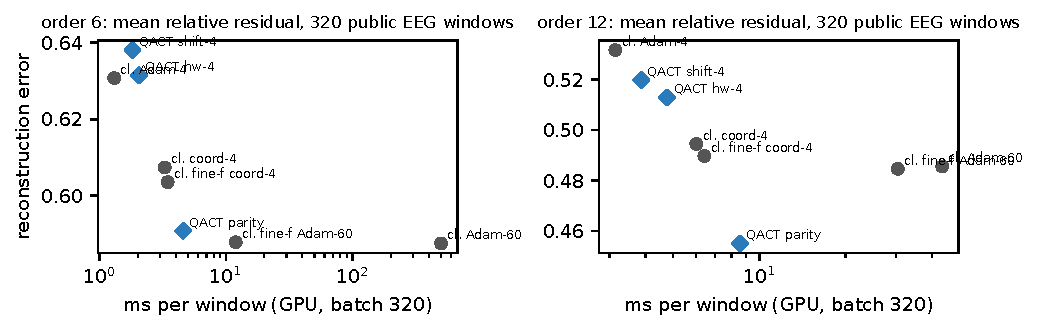
\includegraphics[width=0.9\textwidth]{fig_fair.pdf}
\caption{Reconstruction error against GPU time per window for the engines of Table~\ref{tab:fair} (grey: classical; blue: \qact). At equal refinement rule the classical engine is ahead; the \qact\ parity mean at order 12 is carried by the windows on which the classical seed grid fails (text).}
\label{fig:fair}
\end{figure}

Three things follow. First, at equal refinement rule the classical engine is better than \qact: with the same coordinate search the classical engine is \fairCoordVsHwRelTwelve\% below \qact\ at order 12, better on \fairCoordVsHwBetterTwelve\ of \fairN\ windows ($p=\fairCoordVsHwPTwelve$); the coordinate search itself costs the classical engine \fairClCoordRelTwelve\% against sixty Adam steps at a tenth of the time, consistent with the denoising arm above. Second, the 0.5\,Hz grid changes nothing on this metric at these orders (\fairClFineAdamRelTwelve\% at order 12, $p=\fairClFineAdamPTwelve$); its denoising gain in \S\ref{sec:denoise} is a property of the denoising task, whose mechanism we did not isolate. Third, \qact\ at parity is \fairQParityRelTwelve\% \emph{better} than the reference in the mean at order 12 but better on only \fairQParityBetterTwelve\ of \fairN\ windows, with a median difference of $\fairParityMedianDiffTwelve$: the mean is carried by \fairRefFailTwelve\ windows on which the classical engine leaves more than 90\% of the energy. Those windows are dominated by 60\,Hz mains interference (\fairDriftFailTwelve\% of their energy above 45\,Hz, against \fairDriftOKTwelve\% for the rest), which the classical engine cannot represent from a seed grid that stops at 40\,Hz, while \qact's exact frequency update reads the periodogram peak wherever it is. Extending the classical seed grid to 78\,Hz leaves \fairLowFailTwelve\ such windows, and the classical engine is then \fairLowVsParityRelTwelve\% relative to \qact\ parity, better on \fairLowVsParityBetterTwelve\ of \fairN\ ($p=\fairLowVsParityPTwelve$); with the backfit pass \qact\ has, it is \fairLowBfVsParityRelTwelve\% (better on \fairLowBfVsParityBetterTwelve, $p=\fairLowBfVsParityPTwelve$). Every remaining difference is a band, dictionary or refiner choice the classical engine can make.

\subsection{Downstream: does the representation change what is learned?}
\label{sec:downstream}
The features are 13 energy-weighted aggregates per channel (band fractions, oscillatory versus transient split, spectral centroid and spread, sweep, duration, reconstruction error), invariant to the greedy order, plus per-channel log-RMS and log line length \citep{esteller2001line}. Table~\ref{tab:downstream} summarises the pre-registered comparisons; Appendix~\ref{app:downstream} has the full tables.

\begin{table}[t]
\caption{Downstream comparisons, all pre-registered, patient- or subject-wise folds. ``Gap'' is the best quantum model minus the best classical model unless stated; $p$ is the paired Wilcoxon across patients or subjects.}
\label{tab:downstream}
\centering\small
\resizebox{\textwidth}{!}{%
\begin{tabular}{@{}llrl@{}}
\toprule
task, data & comparison & gap & verdict \\
\midrule
seizure, CHB-MIT (23 patients) & chirplet + amplitude vs amplitude only, logistic regression & $+8.6$ pts & $p=0.0011$, 20/23 patients \\
seizure, Siena (14, held out) & same, two classifiers & $+9.4$, $+13.3$ pts & $p=0.005$, $0.004$: replicates \\
seizure, CHB-MIT & \qact\ (parity engine, sampled) vs classical features, all features + regularisation & $-4.9$, $-4.5$, $-7.2$ pts & $p=0.0006$, $0.0027$, $<10^{-4}$: classical better \\
seizure, Siena & \qact\ (parity engine) vs classical features; with amplitude & $-2.8$, $-1.8$; $-3.6$, $-5.3$ pts & $p=0.0012$ for the last: classical better \\
seizure, CHB-MIT & best quantum classifier vs classical RBF SVM & $-0.5$, $-0.8$ pts & $p=0.19$, $0.61$: parity \\
rest vs arithmetic, EEGMAT (36) & QSVC / projected kernel / re-uploading / hybrid vs logreg & $-1.3$ to $-8.8$ pts & never ahead \\
forecasting, CHB-MIT (23 people) & quantum LSTM vs classical twin (skill) & $-0.005$ & $p=0.086$: none \\
forecasting, CHB-MIT & quantum reservoir vs echo-state network & $-0.007$ & $p=10^{-4}$, ESN wins 20/23 \\
forecasting, CHB-MIT & quantum reservoir vs its zero-coupling twin, 2\,s steps (60\,s steps) & $+0.024$ ($-0.004$) & $p<10^{-4}$, 23/23 ($p=0.23$): resolution-dependent \\
\bottomrule
\end{tabular}}
\end{table}

The chirplet features are the one solid positive result: worth 9--13 accuracy points beyond amplitude features for cross-patient seizure detection, significant on two databases and two classifiers (best absolute accuracy 81.4\% on CHB-MIT with per-patient normalised features, 76.8\% raw; 79.2\% on Siena; an untuned RBF SVM on all features). The quantum transform does not improve that number: under univariate top-$k$ selection \qact\ features led by 1.2 to 3.0 points, never significantly; under all features with regularisation the classical features led; and with the parity engine, measurement-sampled \qact\ is 4.5 to 7.2 points behind on CHB-MIT and 1.8 to 5.3 behind on Siena, because sampling atoms by measurement costs 4--5 points against the argmax on the same engine. Atom-level improvements that are real (the refiner, cubic and skew atoms, measurement as a proposal distribution that halves the error on planted chirplets) produced no downstream gain; the best of them had the best atoms and the worst features, and on real EEG its reconstruction advantage did not exist (0.3797 versus 0.3828), because 1/f EEG has no clean atoms to find. Reconstruction quality and classification value were close to unrelated, three times over. Among the quantum learners, one effect survived its own control, and only at fine time resolution: at 2\,s steps entanglement contributes to the quantum reservoir's forecasting skill for all 23 people, at 60\,s steps it does not, and the reservoir loses to a classical echo-state network of the same readout size at every resolution.

\section{On hardware}
\label{sec:hw}
On a device the bill is circuits $\times$ shots $\times$ two-qubit gates, and the construction as drafted was expensive on all three: the envelope as a $2^n$-way multiplexed rotation with post-selection discarded 43--97\% of shots on real EEG, and a nine-qubit circuit transpiled to 2,027 CZ gates on a heavy-hex IBM Heron target. Three changes, each exact, reduce it (Fig.~\ref{fig:hardware}). \emph{Folding} the envelope into state preparation loads $e\odot r$ directly: no ancilla, no multiplexor, every shot kept (\hwFoldedCZ\ CZ). The \emph{semiclassical} inverse QFT of \citet{griffiths1996semiclassical} measures each qubit as soon as it is final and replaces every controlled phase by a classically controlled single-qubit phase, so the QFT contains no two-qubit gates (\hwSemiclassicalCZ\ CZ; a dynamic circuit). \emph{Window-local registers} use shift covariance, $c(u+t_0)^2=cu^2+2ct_0u+\text{const}$: a Gaussian atom needs a register only as large as its $\pm4\sigma$ support, the offset folds into one linear phase, and the smaller QFT returns the original distribution exactly on every $2^{n-m}$-th bin. A short atom then needs 6 qubits and about 140 CZ gates, and under the Heron noise model its selection survives (selected-atom energy \hwWindowedSel\ on average over widths, 0.99--1.00 for the two short widths) where the baseline never did (\hwBaselineSel). Per atom, branch-and-bound over envelopes with the classical bound $(\sum e|r|)^2/\norm{e}^2$ visits 57\% of the circuits with identical selections, and the three-point refiner replaces 112 evaluations per step by 8: about 80$\times$ fewer circuit executions per atom. Long atoms ($\log\Delta t\ge3.9$) span the window, cannot be shrunk, and lose their selection under noise; what remains for them is state preparation, about 87\% of the two-qubit budget \citep{holmes2020efficient,moosa2023linear}.

\begin{figure}[t]
\centering
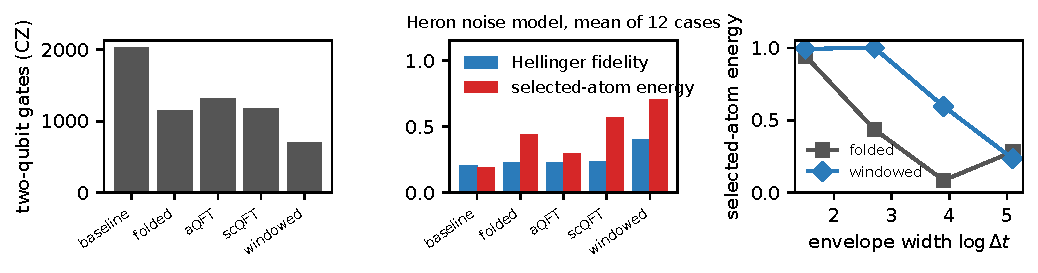
\includegraphics[width=0.9\textwidth]{fig_hardware.pdf}
\caption{Five constructions of the same selection distribution on real EEG windows (12 window $\times$ width cases), transpiled to an IBM Heron target: two-qubit gates, and Hellinger fidelity plus selected-atom energy under the device's calibrated noise model (left, centre); selected-atom energy by envelope width for the folded and windowed constructions (right).}
\label{fig:hardware}
\end{figure}

\paragraph{Real device.} We executed the windowed construction on \texttt{\qpuBackend}, a 156-qubit Heron processor, for \qpuN\ circuits: six public EEG windows (three subjects, two channels) at two short widths, each in the semiclassical (dynamic) form and in a unitary-QFT form that admits gate twirling, plus one long-atom case in both forms, \qpuShots\ shots each with dynamical decoupling (jobs \texttt{\qpuJobs}, \qpuSeconds\ s of processor time). The classical certificate for every circuit is the exact distribution of Proposition~\ref{prop:dequant}. The result splits by register size. The \qpuSixN\ six-qubit circuits (\qpuSixCZ\ CZ on average) selected the exact in-band atom in \qpuSixPeakOK\ cases and the atom they did select carried \qpuSixSel\ of the best atom's energy on average, never less than \qpuSixSelMin: selection survives. The \qpuSevenN\ seven-qubit circuits (\qpuSevenCZ\ CZ) are marginal, with the exact atom in \qpuSevenPeakOK\ cases, a mean of \qpuSevenSel, and \qpuSevenLost\ outright losses. The two nine-qubit long-atom circuits (\qpuLongCZ\ CZ) reached fidelity \qpuLongFid\ and selected-atom energy \qpuLongSel: selection is lost, as the noise model predicted. Measured Hellinger fidelities (\qpuSixFid\ and \qpuSevenFid\ for six and seven qubits) sit below the fake-backend predictions (\qpuSixFidSim\ and \qpuSevenFidSim), so the calibrated model is optimistic by about 0.15--0.2 on this device today; the unitary-QFT form with twirling (\qpuUniFid\ mean fidelity) held up slightly better than the dynamic form without it (\qpuDynFid). Fig.~\ref{fig:device} shows one device histogram against the exact peak and the predicted-versus-measured selection quality for all circuits.

\begin{figure}[t]
\centering
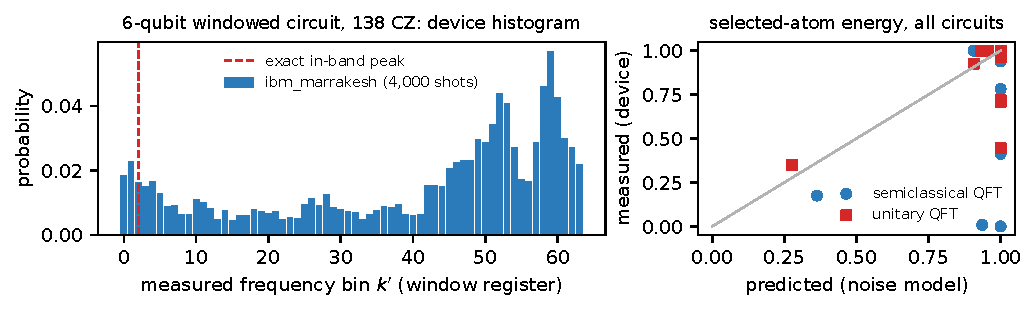
\includegraphics[width=0.9\textwidth]{fig_device.pdf}
\caption{Left: device histogram of a 6-qubit windowed selection circuit on \texttt{\qpuBackend} against the exact distribution; grey bins are out of band (mirror frequencies) and are masked before selection. Right: selected-atom energy predicted by the calibrated noise model against the value measured on the device, all circuits.}
\label{fig:device}
\end{figure}

\paragraph{Speed.} Table~\ref{tab:speed} (Appendix~\ref{app:hw}) prices the same job (four EEGMAT windows, six atoms, OMP) on every engine. On a Heron processor the optimised circuits would take \speedHeron\ per window, and three published techniques (zero repetition delay; multi-programming \speedPack\ circuits per chip, \citealp{niu2023multiprogramming,ohkura2022simultaneous}; adaptive shot allocation by successive elimination, \citealp{huang2025gambling}, run here and cutting shots \speedAdaptiveShots$\times$ at identical error) bring that to \speedAllThree, still about 140$\times$ slower than the classical engine on a CPU and 12,000$\times$ slower than the batched GPU engine. Per shot, the 250\,$\mu$s repetition delay dwarfs the 16--96\,$\mu$s circuit, and each circuit needs thousands of shots to estimate what an FFT computes exactly in microseconds.


\section{Discussion}
\paragraph{What survives.} Three things are genuinely quantum-native in \qact\ and none is an advantage. The frequency axis is free, a constant factor the classical engine buys with a larger grid. The dictionary is gate-native, which removes half of the QRAM assumption in quantum matching pursuit; the signal half remains, and Proposition~\ref{prop:coherent} keeps the residual coherent at the price of a success probability equal to the unexplained energy. The shortest atoms run on today's hardware with the right selection, a statement about circuit design under noise, not speed. Everything else that looked like a win had a classical explanation found by a control: a strong-looking result on real data (17 of 18 subjects, $p<10^{-4}$) was wrong for a reason only the third control revealed, and the pattern recurred for the seed band, twice. \citet{bowles2024better} and \citet{schuld2022quantum} argue that quantum learning needs matched baselines and a goal other than advantage; a representation is where the baseline is easiest to match exactly, since the classical peer is a program, not a model class.

\paragraph{A search that ended negative.} After parity, the study searched for any quantum chirplet transform that beats classical under a criterion fixed in advance: beat the strongest classical baseline, including a classical port of the same idea, in speed at equal accuracy or accuracy at equal time (Appendix~\ref{app:search}). A hybrid transform routed by register size keeps classical quality up to seven qubits and is slower at every level; error correction restores long-atom quality at $6{,}000$--$310{,}000$ physical qubits and 12 minutes to 111 hours per window; a pre-registered 60-window test finds the eight-qubit hybrid indistinguishable from classical and from a noise-mixed classical control; fault-tolerant coherent search crosses over with FFT matching pursuit only at $10^{13}$ atoms; kernels on atoms and small-data regimes land at parity or below; and entangled sensing probes gain nothing at realistic spin numbers, because the brain's own background sets the trial count.

\paragraph{Why no advantage should be expected here.} Recorded signals have to be loaded into every circuit for every shot; that is Aaronson's fine print \citep{aaronson2015fineprint}, and the dequantisation results \citep{tang2019quantum,chia2020sampling} say that once the classical side gets equivalent access the advantage is at most polynomial. Proposition~\ref{prop:dequant} makes it exact for this transform. The exponential advantages published for signals concern signals that reach a qubit directly \citep{huang2022advantage,kannan2026exponential}; an EEG amplifier does not.

\paragraph{Limitations.} The audit covers one transform family, three EEG databases and one device; the hardware runs demonstrate selection for individual circuits, not a full decomposition on a QPU; the coherent-residual construction is verified at $n=6$ with an unoptimised Gaussian preparation; and the learners are those a practitioner would try. Nothing here rules out an advantage for a quantum-native signal.

\section{Conclusion}
A quantum adaptive chirplet transform can be built exactly, refined exactly, brought to full functional parity with a strong classical engine, and run for the shortest atoms on a quantum processor. Under pre-registered comparisons with paired tests on real EEG it is its classical peer's equal and beats nothing; each apparent advantage was a dictionary or seed-band choice the classical engine can copy, and three of the controls that show it are new here. A fully controlled parity, with the controls named before they ran, is the baseline a claimed quantum advantage for recorded signals has to clear.

\subsection*{AI use statement}
An AI assistant (Claude, Anthropic) was used to draft and refactor experiment code, to run and log the reported experiments under the authors' direction, and to edit the manuscript. All experimental design decisions, pre-registered comparisons, claims and interpretations are the authors', who verified every number against the released result files.

\subsection*{Reproducibility statement}
All data are public (PhysioNet). The repository contains the transform, the classical engine, every pre-registered comparison script with its decision rule, the per-window and per-patient result files, the hardware circuit constructions, the device job identifiers and raw counts, and the scripts that regenerate every table, figure and number in this paper from those files (\texttt{paper/iclr2027/exp/}). The three controls added in this paper run in under an hour on one consumer GPU and about 35\,s of QPU time on the IBM open plan.

\subsection*{Ethics statement}
The study uses de-identified public EEG databases under their PhysioNet licences and involves no new human-subject data collection.

\bibliography{refs}
\bibliographystyle{iclr2027_conference}

\appendix
\section{Proofs}
\label{app:proofs}
\paragraph{Proposition~\ref{prop:dequant}.} With $\ket{s}=\sum_t s(t)\ket{t}$ and the conjugate chirp $D_c\ket{t}=e^{-i2\pi ct^2/N}\ket{t}$, the inverse QFT maps $\ket{t}\mapsto N^{-1/2}\sum_k e^{-i2\pi kt/N}\ket{k}$, so the amplitude on $\ket{k}$ is $N^{-1/2}\sum_t s(t)e^{-i2\pi ct^2/N}e^{-i2\pi kt/N}$ and eq.~\eqref{eq:sampler} follows. Writing $\psi_{e,c,k}=e\odot\chi_{c,k}/\norm{e}$ with $\chi_{c,k}(t)=e^{i2\pi(ct^2+kt)/N}$ and using $s=e\odot r/\norm{e\odot r}$, $\braket{\psi_{e,c,k}}{r}=\norm{e}^{-1}\sum_t e(t)r(t)\overline{\chi_{c,k}(t)}=\norm{e\odot r}\norm{e}^{-1}\sum_t s(t)\overline{\chi_{c,k}(t)}$, whose squared modulus is $N\norm{e\odot r}^2\norm{e}^{-2}P_{e,c}(k)$; dividing by $\norm{\psi}^2=1$ gives the claim, and the sum over $t$ for all $k$ is one discrete Fourier transform of $e\odot r\odot e^{-i2\pi ct^2/N}$.

\paragraph{Proposition~\ref{prop:coherent}.} $R_k$ is unitary and Hermitian with $(I+R_k)/2=I-\ket{\psi_k}\bra{\psi_k}=P_k$. On $\ket{0}\ket{r}$, the first Hadamard gives $(\ket{0}+\ket{1})\ket{r}/\sqrt2$, the controlled reflection gives $(\ket{0}\ket{r}+\ket{1}R_k\ket{r})/\sqrt2$, and the second Hadamard gives $\ket{0}\,(I+R_k)\ket{r}/2+\ket{1}\,(I-R_k)\ket{r}/2$; the ancilla reads $0$ with probability $\norm{P_kr}^2/\norm{r}^2$ and leaves $P_k\ket{r}/\norm{P_kr}$. Chaining, $P_K\cdots P_1\ket{x}$ is the matching-pursuit residual $r_K$ because $r_{k}=P_kr_{k-1}$ by definition, and the success probabilities multiply to $\prod_k\norm{r_k}^2/\norm{r_{k-1}}^2=\norm{r_K}^2/\norm{x}^2$. The controlled reflection needs only the reflection about $\ket{0}$ to be controlled: $\mathrm{c}\text{-}R_k=(I\otimes U_k)\,\mathrm{c}\text{-}(I-2\ket{0}\bra{0})\,(I\otimes U_k^\dagger)$, a multi-controlled phase of $\pi$ conjugated by $X^{\otimes n}$.

\begin{figure}[h]
\centering
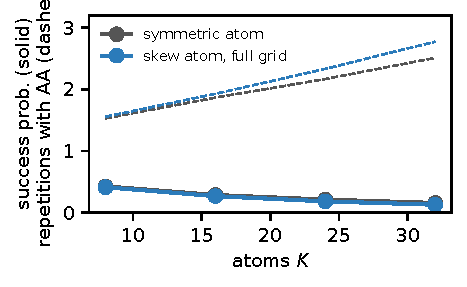
\includegraphics[width=0.42\textwidth]{fig_coherent.pdf}
\caption{Coherent-residual success probability (solid) and repetitions under amplitude amplification (dashed) as a function of the number of atoms, from the mean squared relative residual of the classical study on 320 public EEG windows \citep{actcode}.}
\label{fig:coherent}
\end{figure}

\paragraph{Complexity of the superposed search.} With the triples $(t_c,\Delta t,c)$ in index registers, the envelope preparation and the phase gates of eq.~\eqref{eq:twolocal} become controlled on those registers; the outcome register holds $k$. Quantum maximum finding \citep{durr1996minimum} over $(\text{index},k)$ with the amplitude estimated to precision $\varepsilon$ \citep{brassard2002amplitude} costs $O(\sqrt{M'N_f}\,\varepsilon^{-1})$ preparations of the searched state, each of which loads $x$ ($\Theta(N)$ gates without QRAM) and applies the $k-1$ reflections of Proposition~\ref{prop:coherent} ($O(kn^2)$ plus envelope preparations), giving the bound quoted in \S\ref{sec:theory}. The $N_f$ factor is absorbed into $M'$ in the text.

\section{Refinement control: additional detail}
\label{app:fair}
Table~\ref{tab:fairbf} gives the backfit and extended-band arms. Windows on which the classical engine as shipped leaves more than 90\% of the energy have \fairDriftFailTwelve\% of their energy above 45\,Hz (mains); the others \fairDriftOKTwelve\%.

\begin{table}[h]
\caption{Backfit and extended-band arms, same windows as Table~\ref{tab:fair}: mean and median relative residual at order 12, change versus the classical engine as shipped, windows better, paired $p$.}
\label{tab:fairbf}
\centering\small
\resizebox{\textwidth}{!}{%
\begin{tabular}{@{}lrrrrr@{}}
\toprule
engine & mean@6 & mean@12 & median@12 & vs ref@12 & better / $p$ \\
\midrule
classical, Adam 60 (reference) & \fairBfRefErrSix & \fairBfRefErrTwelve & \fairBfRefMedTwelve & -- & \\
classical + backfit 1 & \fairBfOneErrSix & \fairBfOneErrTwelve & \fairBfOneMedTwelve & \fairBfOneRelTwelve\% & \fairBfOneBetterTwelve\ / $\fairBfOnePTwelve$ \\
classical, seed grid to 78\,Hz & \fairBfLowErrSix & \fairBfLowErrTwelve & \fairBfLowMedTwelve & \fairBfLowRelTwelve\% & \fairBfLowBetterTwelve\ / $\fairBfLowPTwelve$ \\
classical, seed grid to 78\,Hz + backfit 1 & \fairBfLowOneErrSix & \fairBfLowOneErrTwelve & \fairBfLowOneMedTwelve & \fairBfLowOneRelTwelve\% & \fairBfLowOneBetterTwelve\ / $\fairBfLowOnePTwelve$ \\
\qact\ parity & \fairBfParityErrSix & \fairBfParityErrTwelve & \fairBfParityMedTwelve & \fairBfParityRelTwelve\% & \fairBfParityBetterTwelve\ / $\fairBfParityPTwelve$ \\
\bottomrule
\end{tabular}}
\end{table}

\section{Downstream comparisons: full tables}
\label{app:downstream}
\paragraph{Seizure detection.} CHB-MIT: 10,856 two-second epochs (5,501 ictal / 5,355 interictal), 23 patients, cross-patient folds. With all 270 chirplet + amplitude features and regularisation (no selection), the gain of chirplet features over amplitude-only, paired across patients (decision threshold $p<0.0036$): logistic regression $C=0.01$, raw, $+8.6$ points ($p=0.0011$, 20/23); $C=0.1$, raw, $+7.5$ ($p=0.0005$, 20/23); RBF SVM, raw, $+3.4$ ($p=0.050$); logistic $C=0.01$, per-patient normalised, $+3.5$ ($p=0.0096$); $C=0.1$, normalised, $+3.4$ ($p=0.0015$, 17/23); RBF SVM, normalised, $+1.9$ ($p=0.039$), best absolute 81.4\%. Under univariate top-$k$ selection every model selected all 36 amplitude features first and the ``chirplet + amplitude'' result was in fact amplitude-only, which is why the selection regime was replaced. \qact\ versus classical features, all features and regularisation: logistic L2 62.7 vs 63.6\%, L1 62.9 vs 63.4\%, RBF SVM 66.4 vs 67.5\%; sampled versus argmax selection for the SVM $-1.93$ points, $p=0.0032$. Siena (14 patients, 45 seizures, never inspected during development): amplitude only 69.5 / 65.9\% (logistic / SVM), chirplet + amplitude 78.9 / 79.2\%, \qact\ + amplitude 78.5 / 79.1\%; chirplet gain $+9.43$ ($p=0.0047$) and $+13.31$ ($p=0.0040$); \qact\ versus classical $+0.30$ and $-1.99$, not significant.

\paragraph{Quantum classifiers.} CHB-MIT, ACT + amplitude features, pre-registered win = best quantum $>$ best classical and $p<0.025$: RBF SVM 67.7\% raw / 79.2\% per-patient normalised; projected quantum kernel 66.9 / 78.0; QSVC 65.8 / 78.2; quantum-feature logistic regression 63.8 / 78.7; hybrid 63.9 / 76.8 and its no-entanglement twin 63.9 / 76.8; logistic regression 64.5 / 76.1. EEGMAT (rest versus arithmetic, 36 subjects, nested subject-wise CV, equal tuning budgets): logistic regression 55.0 / 57.4\% (raw / per-subject normalised), RBF SVM 51.6 / 55.7, QSVC 53.5 / 54.4, projected kernel 52.7 / 54.3; quantum features with linear readout 52.8 / 56.6 against 54.5 / 57.9 classical; the entangled hybrid 53.1 / 56.5 against its non-entangled twin 54.8 / 57.9. The alpha-suppression effect that validates the loading is present at the recording level ($-25.5\%$, 8/8 subjects, $p=0.0078$) and nearly washes out per epoch.

\paragraph{Forecasting.} Per-person models on the first half of each CHB-MIT recording, tested on the second half (490\,h each), 270 features in 10\,s steps, targets the next minute of features and a seizure-within-5-minutes probability. LSTM skill $+0.106$; fixed quantum-circuit features $+0.101$ against twin $+0.102$; quantum LSTM $+0.014$ against twin $+0.019$. Quantum reservoirs (four parallel 8-qubit disordered transverse-field Ising systems, input-qubit replacement, ridge readout; exact density-matrix simulation verified against a circuit simulator to $10^{-7}$): on NARMA-10 and memory capacity the quantum reservoir beats an echo-state network of the same readout size (0.191 vs 0.240 error; capacity 14.8 vs 11.5); on EEG at 2\,s steps run continuously, ESN $+0.436$, quantum $+0.429$, zero-coupling twin $+0.405$; the entanglement contribution grows monotonically as the step shortens (60\,s: $-0.004$, $p=0.23$; 2\,s: $+0.024$, 23/23, $p<10^{-4}$) and the classical reservoir wins at every step size.

\section{The study's later search for a quantum win}
\label{app:search}
All numbers are from the study's result files (\texttt{results/hybrid\_act\_levels.json}, \texttt{qact\_qec.json}, \texttt{q8\_vs\_classical.json}, \texttt{qsearch\_*.json}, \texttt{quantum\_sensing\_opm.json}) and its search log (\texttt{docs/QACT\_SEARCH\_LOG.md}). \emph{Hybrid levels} (4 EEGMAT windows, 6 atoms, quantum routes executed under the Heron noise model): fit error 0.578 classical; 0.575, 0.567, 0.561 at levels q6--q8 (2--21\% of evaluations quantum, chosen atoms at 99--91\% of the best on average, worst 80--54\%); 0.734 at q9 (all quantum, worst atom 31\%); every level slower than the 45\,ms classical run. \emph{Error correction} (Microsoft resource estimator, surface code, logical-level runs in Aer): Heron as calibrated is above threshold on readout error; with $10^{-3}$ or $10^{-4}$ physical error rates q8/q9 recover their noiseless quality (0.573/0.598) at 6,480--95,256 physical qubits and 12 minutes to 4.8 hours per window; with perfect qubits q9 remains slightly worse than classical (0.598 vs 0.578) from shot noise and coarser window grids. \emph{Powered test} (60 fresh windows, 30 subjects, paired Wilcoxon, $\alpha=0.0125$): q8 on Heron $+0.0007$ ($p=0.79$), error-corrected $+0.0016$ ($p=0.077$), classical noise-mixed controls $-0.0022$ and $+0.0008$, noiseless q8 $+0.0063$ ($p=0.0014$, worse). \emph{Fault-tolerant coherent search}: Dürr--Høyer with amplitude estimation, every constant tilted toward quantum and QRAM free, crosses over with classical FFT matching pursuit at $1.5\times10^{13}$ atoms. \emph{Learners on chirplet atoms} (CHB-MIT, patient-wise): a quantum kernel on sets of atoms 62.6\% vs 67.4\% RBF-SVM ($p=0.0015$), an all-feature kernel 74.8\% vs 76.8\% ($p=0.09$), learning curves from 20 to 200 training epochs at parity once kernel concentration was controlled. \emph{Sensing}: on real OPM-MEG evoked fields a noiseless sensor needs only 1.1--2.3$\times$ fewer trials than today's OPM, and entangled probes gain $\ge10\%$ only below $3\times10^{9}$ spins with $T_2\ge1$\,s.

\section{Hardware details}
\label{app:hw}
\begin{table}[h]
\caption{Time per window for the same decomposition job. Device rows price the circuits the simulator run actually executed, at the device's calibrated gate and measurement durations; queueing and compilation excluded.}
\label{tab:speed}
\centering\small
\resizebox{\textwidth}{!}{%
\begin{tabular}{@{}lrrr@{}}
\toprule
engine & per window & vs classical CPU & recon.\ error \\
\midrule
classical engine, GPU, batch 1,024 & \speedClGPUBatched & 82$\times$ faster & \speedClGPUErr \\
classical engine, CPU & \speedClCPU & -- & \speedClCPUErr \\
\qact\ exact simulation, GPU, batch 1,024 (the dequantised program) & \speedQSimBatched & 630$\times$ faster & \speedQSimErr \\
\qact\ circuits shot by shot, simulator (\speedCircuitsPerWindow\ circuits) & \speedQAer & 971$\times$ slower & \speedQAerErr \\
IBM Heron, optimised circuits (estimate) & \speedHeron & 13,700$\times$ slower & \\
\quad + zero repetition delay, multi-programming, adaptive shots & \speedAllThree & 144$\times$ slower & \\
IBM Heron, original design (estimate) & \speedHeronOrig & $1.1\times10^6\times$ slower & \\
\bottomrule
\end{tabular}}
\end{table}

Circuits are built from Qiskit library components (\texttt{StatePreparation}, \texttt{QFTGate}, \texttt{UCRYGate}) and transpiled with the preset pass manager at optimisation level 3 to the device target (heavy-hex coupling, native CZ, RZ, SX, X, mid-circuit measurement and feed-forward). Gate counts in Fig.~\ref{fig:hardware} are from a Heron target; noisy simulation uses that backend's calibrated noise model. The device run used \texttt{\qpuBackend} through the open plan with dynamical decoupling (XY4) on both jobs and gate and measurement twirling (16 randomisations) on the unitary-QFT job; the dynamic-circuit job could not be twirled. The exact target for every circuit, its transpiled gate counts, the fake-backend prediction, the device counts and the job identifiers are in \texttt{paper/iclr2027/results/}.

\end{document}
